\documentclass[main.tex]{subfiles}

\begin{document}
\chapter{Ab initio methods for materials modeling}\label{chap:ab-initio-modeling}

%\section{The electronic structure problem\label{sec:theory_schrödinger}}

The description of matter by theoretical methods starts from the Hamiltonian of an interacting system of electrons and nuclei (with electrons coordinates \(\vb*{r}_i\) and nuclei coordinates \(\vb*{R}_{\alpha}\))
\begin{align}
    \ope{H} &= \ope{T}_{\mathrm{e}} + \ope{U}_{\mathrm{e-e}} + \ope{T}_{\mathrm{n}} + \ope{V}_{\mathrm{n-e}} + \ope{W}_{\mathrm{n-n}} \\
    &= - \sum_i \frac{1}{2} \nabla^2_i 
    + \frac{1}{2} \sum_{i \neq j} \frac{1}{\vert \vb*{r}_i - \vb*{r}_j \vert} 
    - \sum_{\alpha} \frac{1}{2 M_{\alpha}} \nabla^2_{\alpha}
    - \sum_{i, \alpha} \frac{Z_{\alpha}}{\vert \vb*{r}_i - \vb*{R}_{\alpha} \vert} 
    + \frac{1}{2} \sum_{\alpha \neq \beta} \frac{Z_{\alpha} Z_{\beta}}{\vert \vb*{R}_{\alpha} - \vb*{R}_{\beta} \vert}
\end{align}
where
\begin{itemize}
    \item \(\ope{T}_{\mathrm{e}}\,, \ope{T}_{\mathrm{n}}\) are the kinetic energies of the electrons and nuclei respectively,
    \item \(\ope{U}_{\mathrm{e-e}}\) is the Coulomb interaction between the electrons,
    \item \(\ope{V}_{\mathrm{n-e}}\) is the Coulomb interaction between the electrons and the nuclei,
    \item \(\ope{W}_{\mathrm{n-n}}\) is the Coulomb interaction between the nuclei.
\end{itemize}
This very general problem consisting of both the electronic and nucleic degrees of freedom can be simplified in a first step by employing the Born-Oppenheimer approximation \cite{born_zur_1927}.
The approximation assumes the nuclei to be fixed point charges which create a potential for the \(N\) interacting electrons, so that the electronic part can be solved independently using the nuclei positions as a parameter
\begin{align}
    \ope{H}_{\mathrm{BO}} &= \ope{T}_{\mathrm{e}} + \ope{U}_{\mathrm{e-e}} + \ope{V}_{\mathrm{n-e}} + \ope{W}_{\mathrm{n-n}} \\
    &= -\sum_i \frac{1}{2} \nabla^2_i 
    + \frac{1}{2} \sum_{i \neq j} \frac{1}{\vert \vb*{r}_i - \vb*{r}_j \vert} 
    - \sum_i \sum_{\alpha} \frac{Z_{\alpha}}{\vert \vb*{r}_i 
    - \vb*{R}_{\alpha} \vert} 
    + \frac{1}{2} \sum_{\alpha \beta} \frac{Z_{\alpha} Z_{\beta}}{\vert \vb*{R}_{\alpha} - \vb*{R}_{\beta} \vert}\,. \label{eq:bo_hamiltonian}
\end{align}
The terms \(\ope{V}_{n-e}\) and \(\ope{W}_{n-n}\) here are just a function of the electronic coordinates \(\vb*{r}\) and a constant respectively. Hence they can then be combined into a potential \(\ope{V} (\vb*{r})\) for the interacting electrons and the Hamiltonian reads
\begin{equation}\label{eq:solid_state_hamiltonian}
    \ope{H} = \ope{T} + \ope{U} + \ope{V}\,.
\end{equation}

\section{Density Functional Theory\label{sec:theory_dft}}

Obtaining solutions to the Schrödinger equation with the Hamiltonian \ref{eq:bo_hamiltonian} is analytically impossible, as it produces a system of \(3N\) coupled differential equations, with \(N \sim N_{\mathrm{Avogadro}} \sim \mathcal{O} (10^{23})\).
As such, the need for good approximations to obtain results for real world
systems is high.
One particularly successful approach is \acrfull{dft}.
In the following section, the theoretical framework of \acrshort{dft} will be reviewed following the PhD thesis of Nicola Marzari \cite{marzari_ab-initio_1996}, a more extensive discussion can be found in Richard Martins textbook on electronic structure \cite{martin_electronic_2004}.

\subsection{Hohenberg-Kohn theorems}

The start for DFT is the exact reformulation of the electronic structure problem by Hohenberg and Kohn.
This reformulation uses the ground state density of the electronic system \(n_0 (r)\) as the basic variable.
To achieve this, Hohenberg and Kohn formulated two theorems \cite{hohenberg_inhomogeneous_1964}, which demonstrate that the ground state properties of an electronic system can be described using the ground state density (the proof of those theorems is omitted here, but can be found in the original publication \cite{hohenberg_inhomogeneous_1964} or the textbook by Martin \cite[chapter 6.2]{martin_electronic_2004}):
\begin{enumerate}[I]
    \item The external potential is a unique functional of the ground state density.
    \item The ground state energy minimizes the energy functional,
    \[E[n(\vb*{r})] > E_0 \;\forall\; n(\vb*{r}) \neq n_0 (\vb*{r})\,.\]
\end{enumerate}
These theorems proof the existence and uniqueness of the energy functional \(E[n(\vb*{r})]\), but a concrete expression for it cannot be given.
As the ground state wave function is a functional of the ground state density, a formal definition of the energy functional can be written as
\begin{align*}
    E[n(\vb*{r})] &= \expval{\ope{H}}{\Psi} \\
    &= \expval{\ope{T} + \ope{U} + \ope{V}}{\Psi} \\
    &= \expval{\ope{T} + \ope{U}}{\Psi} + \int \dd{\vb*{r}^{\prime}} \Psi^* (\vb*{r}^{\prime}) V(\vb*{r}^{\prime}) \Psi (\vb*{r}^{\prime})\,.
\end{align*}
Defining the universal functional \(F[n(\vb*{r})] = \expval{T + U}{\Psi}\), which is material independent and writing \(n (\vb*{r}^{\prime}) = \Psi^* (\vb*{r}^{\prime}) \Psi (\vb*{r}^{\prime})\), the energy functional becomes
\begin{equation}\label{eq:hohenberg_kohn_energy_functional}
    E[n(\vb*{r})] = F[n(\vb*{r})] + \int \dd{\vb*{r}^{\prime}} V(\vb*{r}^{\prime}) n (\vb*{r}^{\prime})\,.
\end{equation}
This is just a formal definition, as all the formerly mentioned complication of the Hamiltonian \ref{eq:solid_state_hamiltonian} now lies in the functional \(F[n(\vb*{r})]\).
With a known or well approximated universal functional \(F[n(\vb*{r})]\), the Hohenberg-Kohn theorems provide a great simplification for finding the ground state properties of a solid state system, as the problem is now only a variational problem with 3 spatial coordinates instead of \(3N\) coordinates when trying to solve the full Hamiltonian.


\subsection{Kohn-Sham equations}

Kohn and Sham proposed an approach for handling interacting many-body systems by introducing an auxiliary non-interacting system of electrons \cite{kohn_self-consistent_1965}
\begin{equation}\label{eq:kohn_sham_hamiltonian}
    H_0 = \sum_i^{N_e} \frac{p_i^2}{2m} + v_{\mathrm{KS}} (\vb*{r}_i)\,.
\end{equation}
With a correction potential \(v_{\mathrm{KS}}\) such that the ground state charge density for the auxiliary and the interacting system are the same.
This introduces a new set of orthonormal wave functions, the solutions to the non-interacting problem \(\psi_i\).
The density for this system is calculated as
\begin{equation}\label{eq:density_ks_states}
    n(\vb*{r}) = \sum_{i=1}^{\nicefrac{N_{\mathrm{e}}}{2}} \vert \psi_i (\vb*{r}) \vert^2\,.
\end{equation}
The restriction of equality of the ground state densities for the interacting and the non-interacting system makes it possible to calculate all properties of the interacting system just by solving the non-interacting system (using the Hohenberg-Kohn theorems).
This connection is visualized in a flowchart in fig. \ref{fig:kohn_sham_dft_schema}.
The important point is that in principle, all many-body properties are available through the \gls{kohn_sham} scheme.
\begin{figure}
    \centering
    \begin{subequations}
    \begin{empheq}[box=\widefbox]{align*}
        V (\vb*{r}) & \hspace{1cm} \stackrel{\mathclap{\normalfont\mbox{HK}}}{\impliedby} &  n_0 (\vb*{r}) & \hspace{1cm}\stackrel{\mathclap{\normalfont\mbox{KS}}}{\iff} & n_0 (\vb*{r}) & \hspace{1cm}\stackrel{\mathclap{\normalfont\mbox{HK}}}{\implies} & v_{\mathrm{KS}} (\vb*{r}) \\
        \Downarrow & & \Uparrow & & \Uparrow & & \Downarrow \\
        \Psi_i (\vb*{r}) & \hspace{1cm} \implies &  \Psi_0 (\vb*{r}) & & \psi_i (\vb*{r}) & \hspace{1cm}\impliedby & \psi_i (\vb*{r})
    \end{empheq}
    \end{subequations}
    %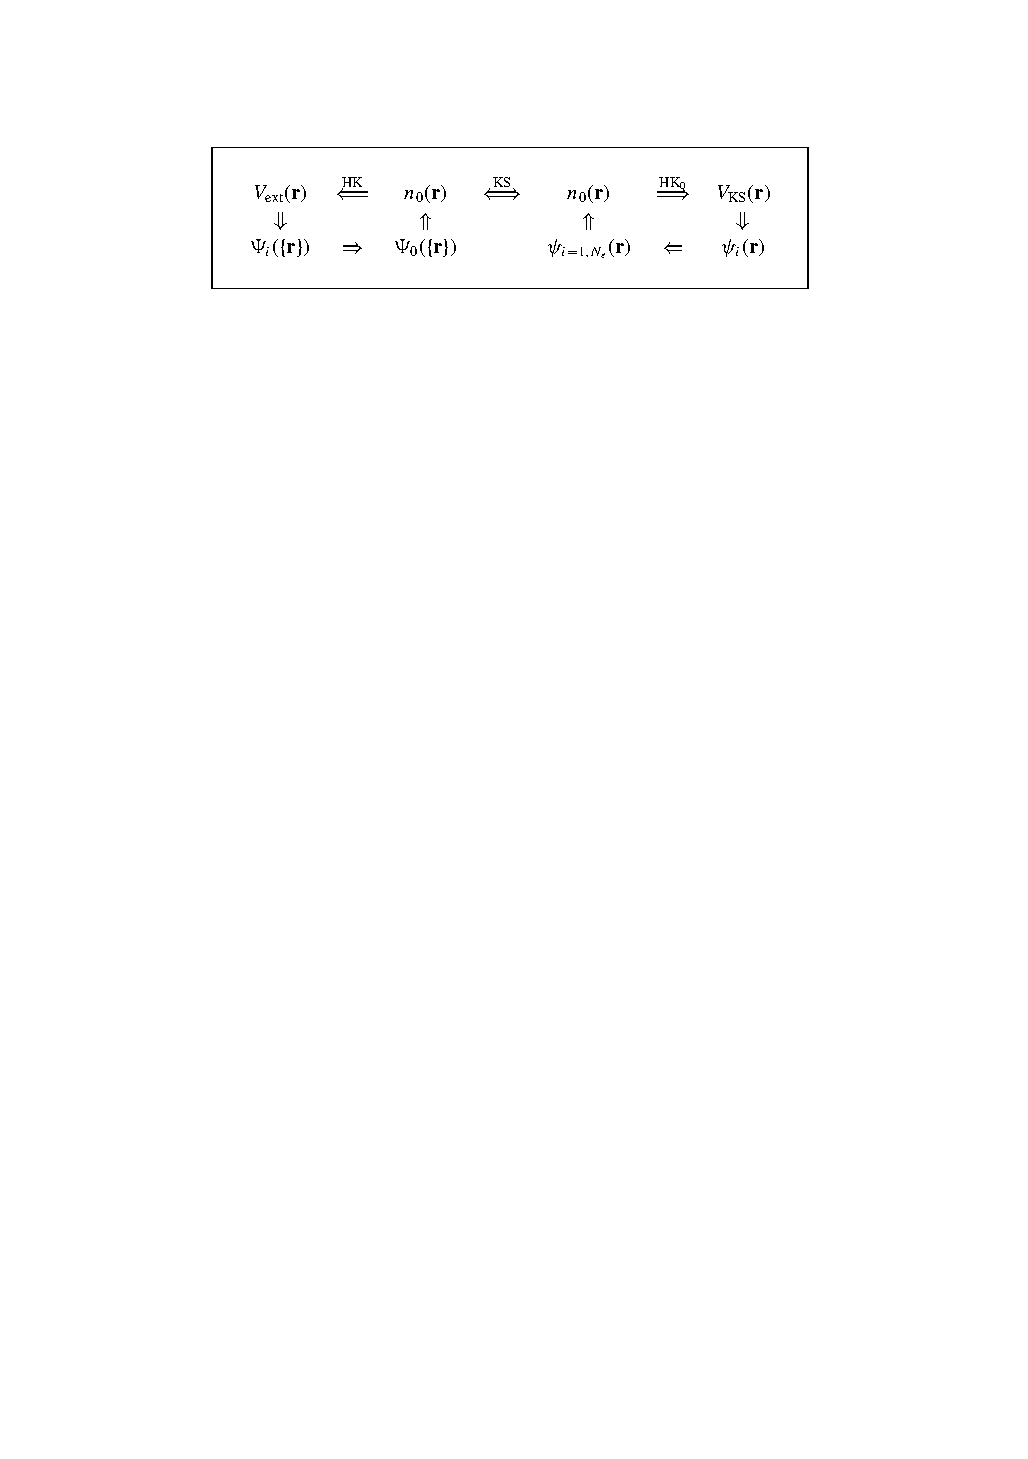
\includegraphics[width=0.7\textwidth]{martins_ks_dft_schema.pdf}
    \caption{Representation of the \acrshort{kohn_sham} ansatz. This scheme shows the connection between many-body properties (left) and the auxiliary \acrshort{kohn_sham} system (right). \(\mathrm{HK}\) here denotes the Hohenberg-Kohn theorems applied to the respective system. The schema is taken from \cite[137]{martin_electronic_2004} and adapted for the notation in this thesis.}
    \label{fig:kohn_sham_dft_schema}
\end{figure}

The kinetic energy of such a non-interacting problem can be easily calculated as sum over all electrons
\begin{equation}
    T_{\mathrm{S}} [n(\vb*{r})] = - \frac{1}{2} \sum_{i=1}^{N_{\mathrm{e}} / 2} \int \dd[3]{r} \psi_i^* (\vb*{r}) \Delta \psi_i (\vb*{r})\,.
\end{equation}
With the help of this system and the classical electrostatic energy 
\begin{equation}
    E_{\mathrm{H}} [n(\vb*{r})] = \frac{1}{2} \int \int \dd[3]{r_1} \dd[3]{r_2} \frac{n(\vb*{r}_1) n(\vb*{r}_2)}{\vert \vb*{r}_1 - \vb*{r}_2 \vert}\,,
\end{equation}
an ansatz for the total energy functional in eq. \ref{eq:hohenberg_kohn_energy_functional} can be written as
\begin{equation}
    E[n(\vb*{r})] = T_{\mathrm{S}} [n(\vb*{r})] + E_{\mathrm{H}} [n(\vb*{r})] + E_{\mathrm{XC}} [n(\vb*{r})] + \int \dd{\vb*{r}^{\prime}} V(\vb*{r}^{\prime}) n (\vb*{r}^{\prime})\,.
\end{equation}
where now \(E_{\mathrm{XC}} [n(\vb*{r})]\) is a functional of the density accounting for all exchange and correlation effects not present in the non-interacting electron system.
The success of \acrshort{dft} lies in the fact that \(E_{\mathrm{XC}}\) contributes only a small part of the total energy and can be approximated in a useful manner. 
Even very simple approximations to \(E_{\mathrm{XC}}\) such as the Local Density Approximation (LDA), which uses the exchange and correlation energy of a homogenous electron gas can give accurate results for very inhomogeneous systems \cite{harris_adiabatic-connection_1984}.

Using that form of \(E[n(\vb*{r})]\), from the variational problem (with a Lagrange parameter introduced to ensure the orthonormality of the states \(\psi_i\))
\begin{align}
     \delta \left( E [n(\vb*{r})] - \sum_j \lambda_j \left[\int \dd[3]{r} \vert \psi_j \vert^2 - 1 \right] \right) = 0
\end{align}
a set of single particle, Schrödinger-like equations can be derived:
\begin{equation}\label{eq:kohn-sham-equations}
    \left(-\frac{1}{2} \Delta + \frac{1}{2} \int \dd[3]{r^{\prime}} \frac{n(\vb*{r}^{\prime})}{\vert \vb*{r} - \vb*{r}^{\prime} \vert} + \fdv{E_{\mathrm{XC}}}{n(\vb*{r})} + V\right) \psi_i (\vb*{r}) = \lambda_i \psi_i (\vb*{r})
\end{equation}
Schrödinger-like in this context means, that with the identification of the Hartree potential \(V_{\mathrm{H}} = \frac{1}{2} \int \dd[3]{r^{\prime}} \frac{n(\vb*{r}^{\prime})}{\vert \vb*{r} - \vb*{r}^{\prime} \vert}\) and the exchange-correlation potential \(V_{\mathrm{XC}} = \fdv{E_{\mathrm{XC}}}{n(\vb*{r})}\) the potential \(v_{\mathrm{KS}}\) in eq. \ref{eq:kohn_sham_hamiltonian} is
\begin{equation}
    v_{\mathrm{KS}} =  V_{\mathrm{H}} + V_{\mathrm{XC}} + V = \frac{1}{2} \int \dd[3]{r^{\prime}} \frac{n(\vb*{r}^{\prime})}{\vert \vb*{r} - \vb*{r}^{\prime} \vert} + \fdv{E_{\mathrm{XC}}}{n(\vb*{r})} + V\,.
\end{equation}
Eq. \ref{eq:kohn-sham-equations} can be rewritten as the \acrshort{kohn_sham} equations
\begin{equation}
    \left(- \frac{1}{2} \Delta + v_{\mathrm{KS}}\right) \psi_i (\vb*{r}) = \epsilon_i \psi_i (\vb*{r})\,.
\end{equation}
Importantly, the potential \(v_{\mathrm{KS}}\) depends on the solutions \(\psi_i (\vb*{r})\), as \(V_{\mathrm{H}}\) and \(V_{\mathrm{XC}}\) include the density \(n(\vb*{r})\).
The problem thus is a self-consistent problem, meaning the density used for calculating the potentials and the obtained solution only agree for the exact solution.
Arriving at a solution consists then of iterating the process of obtaining a new set of potentials from the solution and solving the \acrshort{kohn_sham} equations again.

This kind of iterative, self-consistent method lends itself to being implemented in a computational context, as every single step is mathematically simple and the complexity arises for instance from size of the matrices occurring or the number of steps needed, which makes calculation by hand tedious but is perfectly suited for execution on a computer.

\subsection{Pseudopotentials and basis set}\label{sub:theory_basis_set}

In order to represent the states and operators in eq. \ref{eq:kohn-sham-equations}, a basis set has to be chosen.
Bloch's theorem states that in case of a periodic external potential, which makes the Hamiltonian commute with translation operators for translation by a lattice vector, the common eigenstates of these operators are:
\begin{equation}
    \psi (\vb*{r}) = \psi_{n \vb*{k}} (\vb*{r}) = e^{i \vb*{k} \cdot \vb*{r}} u_{n \vb*{k}} (\vb*{r})\,,
\end{equation}
where \(\vb*{k}\) is the quasi-momentum, \(n\) is the band index and \(u_{n \vb*{k}} (\vb*{r})\) has the periodicity of the unit cell.
A natural choice to represent \(u_{n \vb*{k}} (\vb*{r})\) is the discrete set of plane waves
\begin{align}
    u_{n \vb*{k}} (\vb*{r}) &= \frac{1}{\sqrt{V}} \sum_{\vb*{G}} e^{i \vb*{G} \vb*{r}}\,,
\end{align}
where \(\vb*{G}\) is a reciprocal lattice vector and \(V\) is the volume of the unit cell.
From that the form \(\psi_{n \vb*{k}}\) follows:
\begin{align}\label{}
    \implies \psi_{n \vb*{k}} (\vb*{r}) &= \frac{1}{\sqrt{V}} \sum_{\vb*{G}} e^{i (\vb*{k} + \vb*{G}) \vb*{r}}\,.
\end{align}
With this choice of basis set, the kinetic energy is easily calculated:
\begin{equation}
    \bra{\psi_{n \vb*{k}} (\vb*{r})} - \nabla^2 \ket{\psi_{n \vb*{k}} (\vb*{r})} = \sum_{\vb*{G}} c_{n \vb*{k}, \vb*{G}}^2 \vert \vb*{k} + \vb*{G} \vert^2\,.
\end{equation}
\todo{this is still weird with the expansion coefficent c}
Another important consequence of this choice of basis set is that the electron density (eq. \ref{eq:density_ks_states}) now becomes an integral over the Brillouin zone, which for numerical computation has to be approximated by a sum over a finite set of \(k\) points. \todo{concrete formula for that?}

One problem of this choice of basis set lies in the fact that the lower energy core electrons are localized in the unit cell and as such need a significant amount of plane waves to be meaningfully described.

Importantly, the core electrons don't contribute directly to chemical bonds and physical properties of a solid, only by interaction with valence electrons.
An approach to make the calculations more economically is to then not treat the core electrons explicitly, but instead to introduce an effective potential which includes the effects of both the core and the core electrons.
These potentials are called \acrfull{pp}.
They can be constructed from precise atomical calculations and significantly reduce the number of basis functions required while keeping the calculations accurate.

A \emph{cutoff energy} \(E_{\mathrm{cutoff}}\) can be used to further reduce computation time by allowing only expansion coefficient with 
\begin{equation}
    \frac{\vert \vb*{k} + \vb*{G} \vert^2}{2} \leq E_{\mathrm{cutoff}}\,.
\end{equation}

With Fast Fourier Transforms \gls{fft}, an efficient algorithm exists to transform from (discrete) real to (discrete) reciprocal space.
Every expectation value can be calculated in the optimal representation: in reciprocal space for the kinetic energy and in real space for the pseudopotentials.
Details about the implementation of this will be discussed in sec. \ref{sub:qe_parallelization}.

\section{Density Functional Perturbation Theory}\label{sec:theory_dfpt}

Within the framework of \acrshort{dft} a treatment of lattice vibrations can also be derived, as only knowledge of the ground-state density and its linear response to change in nucleic geometry is needed.
Since this is the fundamental quantity in \acrshort{dft}, an extension in \acrshort{dfpt} can be developed for calculating properties of lattice vibrations.
This theory will be outlined in this section, following the review article by Baroni et al. \cite{baroni_phonons_2001}.

\subsection{Sternheimer equation and Hellman-Feynman theorem}

In a first step, two prerequisite equations are derived, namely the Sternheimer equation describing corrections to a wave function and the Hellman-Feynman theorem linking the derivative of the total energy of a system to the derivative of the Hamiltonian with regards to the same parameter.

The Sternheimer equation follows from perturbation theory.
The idea is to treat a quantum system as an easily solvable system \(\ope{H}_0\) experiencing a small perturbation \(\ope{H}_1\).
The Hamiltonian for the perturbed system is then
\begin{equation}
    \ope{H} = \ope{H}_0 + \lambda \ope{H}_1
\end{equation}
with eigenstates und eigenvalues
\begin{equation}\label{eq:dfpt_perturbation_schrödinger}
    \ope{H} \ket{n} = \epsilon_n \ket{n}\,.
\end{equation}
These eigenstates and eigenvalues can now be expanded in terms of the parameter \(\lambda\),
\begin{align}
    \ket{n} &= \ket{n^{0}} + \lambda \ket{n^{1}} + \lambda^2 \ket{n^{2}} + \ldots\,, \\
    \epsilon_n &= \epsilon_n^{(0)} + \lambda \epsilon_n^{(1)} + \lambda^2 \epsilon_n^{(2)} + \ldots\,.
\end{align}
Inserting these expansion into eq. \ref{eq:dfpt_perturbation_schrödinger} and sorting by order of \(\lambda^n\) gives then
\begin{align}
    \text{0\textsuperscript{th} order: }\; &H_0 \ket{n^{0}} = \epsilon_n^{(0)} \ket{n^{0}} \\ 
    \text{1\textsuperscript{st} order: }\; &H_0 \ket{n^{1}} + H_1 \ket{n^{0}} = \epsilon_n^{(1)} \ket{n^{0}} + \epsilon_n^{(0)} \ket{n^{1}} \label{eq:dfpt_perturbation_first_order} \\
    \text{2\textsuperscript{nd} order: }\; &H_0 \ket{n^{2}} + H_1 \ket{n^{1}} = \epsilon_n^{(0)} \ket{n^{2}} + \epsilon_n^{(1)} \ket{n^{1}} + \epsilon_n^{(2)} \ket{n^{0}} \\
    &\hspace{3cm} \vdots \nonumber
\end{align}
Closing the scalar product in eq. \ref{eq:dfpt_perturbation_first_order} with \(\bra{n^{0}}\) from the left leads to the first order energy correction via
\begin{align}
    \bra{n^{0}} H_0 \ket{n^{1}} + \bra{n^{0}} H_1 \ket{n^{0}} &= \epsilon_n^{(1)} \bra{n^{0}} \ket{n^{0}} + \epsilon_n^{(0)} \bra{n^{0}} \ket{n^{1}} \\
    \implies \epsilon_n^{(1)} &= \bra{n^{0}} H_1 \ket{n^{0}}\,.
\end{align}
The first order correction to the eigenstates, also known as the \emph{Sternheimer equation} can be calculated by rearranging eq. \ref{eq:dfpt_perturbation_first_order}
\begin{equation}\label{eq:dfpt_sternheimer}
    (H_0 - \epsilon_n^{(0)}) \ket{n^1} = -(H_1 - \epsilon_n^{(1)}) \ket{n^0}\,.
\end{equation}

The Hellman-Feynman theorem \cite{feynman_forces_1939} links the derivative of the eigenvalue of a Hamiltonian \(\ope{H}_{\lambda}\) depending on a continuos parameter \(\lambda\) with the derivative of the Hamiltonian with respect to that same parameter.
Starting from the Schrödinger equation
\begin{equation}
    \ope{H}_{\lambda} \ket{\psi_{\lambda}} = E_{\lambda} \ket{\psi_{\lambda}}
\end{equation}
the derivative of \(E_{\lambda}\) with respect to \(\lambda\) can be calculated using the product rule
\begin{align}
    \pdv{E_{\lambda}}{\lambda} &= \pdv{\lambda} \bra{\psi_{\lambda}} \ope{H}_{\lambda} \ket{\psi_{\lambda}} \\
    &= \bra*{\pdv{\psi_{\lambda}}{\lambda}} \ope{H}_{\lambda} \ket{\psi_{\lambda}} + \bra{\psi_{\lambda}} \ope{H}_{\lambda} \ket*{\pdv{\psi_{\lambda}}{\lambda}} + \bra{\psi_{\lambda}} \pdv{\ope{H}_{\lambda}}{\lambda} \ket{\psi_{\lambda}}\,.
\end{align}
\(\ope{H}_{\lambda}\) can now act on the states \(\ket{\psi_{\lambda}}\) to the right or to the left in the first two terms
\begin{align}
    &= E_{\lambda} \bra*{\pdv{\psi_{\lambda}}{\lambda}} \ket{\psi_{\lambda}} + E_{\lambda} \bra{\psi_{\lambda}} \ket*{\pdv{\psi_{\lambda}}{\lambda}} + \bra{\psi_{\lambda}} \pdv{\ope{H}_{\lambda}}{\lambda} \ket{\psi_{\lambda}} \\
    &= E_{\lambda} \pdv{\lambda} \braket{\psi_{\lambda}} + \bra{\psi_{\lambda}} \pdv{\ope{H}_{\lambda}}{\lambda} \ket{\psi_{\lambda}} \\
    &= E_{\lambda} \pdv{\lambda} 1 + \bra{\psi_{\lambda}} \pdv{\ope{H}_{\lambda}}{\lambda} \ket{\psi_{\lambda}}\,.
\end{align}
With that the \emph{Hellman-Feynman theorem} follows:
\begin{equation}\label{eq:dfpt_hellman_feynman}
    \pdv{E_{\lambda}}{\lambda} = \bra{\psi_{\lambda}} \pdv{\ope{H}_{\lambda}}{\lambda} \ket{\psi_{\lambda}}
\end{equation}

\subsection{Lattice vibrations from electronic structure}

As discussed in the beginning of this chapter, nucleic and electronic degrees of freedom can be decoupled in the Born-Oppenheimer approximation.
The connection between lattice dynamics and the electronic structure in the Born-Oppenheimer approximation was first pointed out by De Cicco and Johnson  \cite{decicco_quantum_1969} and Pick, Cohen, and Martin \cite{pick_microscopic_1970}.
The lattice dynamics are determined by
\begin{equation}
    \left( - \sum_{\alpha} \frac{1}{2 M_{\alpha}} \nabla^2_{\alpha} + E(\vb*{R}) \right) \Phi (\vb*{R}) = \mathcal{E} \Phi (\vb*{R})\,,
\end{equation}
where \(\vb*{R}\) is the set of all nuclear coordinates \(\vb*{R}_{\alpha}\) and \(E(\vb*{R})\) is the ground-state energy of the electronic Hamiltonian \ref{eq:bo_hamiltonian}, which depends parametrically on \(\vb*{R}\).
The system is then in equilibrium, when the forces acting on the nuclei vanish
\begin{equation}
    \vb*{F}_{\alpha} = - \pdv{E(\vb*{R})}{\vb*{R}_{\alpha}} = 0\,.
\end{equation}
The vibrational frequencies \(\omega\) are determined by the Hessian of \(E(\vb*{R})\), usually called the matrix of interatomic force constants:
\begin{equation}
    \det \left\vert \frac{1}{\sqrt{M_{\alpha} M_{\beta}}} \pdv{E(\vb*{R})}{\vb*{R}_{\alpha}}{\vb*{R}_{\beta}} - \omega^2 \right\vert = 0\,.
\end{equation}
Thus, the calculation of the vibrational properties as well as the equilibrium geometry depend on the first and second derivatives of the energies \(E(\vb*{R})\).
These derivatives can be calculated using the Hellman-Feynman theorem \ref{eq:dfpt_hellman_feynman}, where the parameter \(\lambda\) is the nucleic coordinate \(\vb*{R}_{\alpha}\). 
Keeping in mind that in the Born-Oppenheimer Hamiltonian \ref{eq:bo_hamiltonian} only the Coulomb interaction between the electrons and the nuclei and the Coulomb interaction between the nuclei have a dependence on the nucleic coordinates \(\vb*{R}\), the force acting on nucleus \(\alpha\) is then
\begin{align}
    \vb*{F}_{\alpha} = - \pdv{E(\vb*{R})}{\vb*{R}_{\alpha}} &= - \mel**{\psi_{\vb*{R}}(\vb*{r})}{\pdv{\ope{H}_{\mathrm{BO}} (\vb*{R})}{\vb*{R}_{\alpha}}}{\psi_{\vb*{R}}(\vb*{r})} \\
    &= - \mel**{\psi_{\vb*{R}}(\vb*{r})}{\pdv{\ope{V}_{\mathrm{n-e}}}{\vb*{R}_{\alpha}} + \pdv{\ope{W}_{\mathrm{n-n}}}{\vb*{R}_{\alpha}}}{\psi_{\vb*{R}}(\vb*{r})} \\
    &= - \int \dd{\vb*{r}} n_{\vb*{R}} (\vb*{r}) \pdv{V_{\vb*{R}} (\vb*{r})}{\vb*{R}_{\alpha}} - \pdv{W_{\mathrm{n-n}}}{\vb*{R}_{\alpha}}\,,
\end{align}
where \(n_{\vb*{R}} (\vb*{r})\) is the ground state electronic density corresponding to a nucleic configuration \(\vb*{R}\).
The second derivative of \(E(\vb*{R})\) is then calculated using the product rule
\begin{equation}\label{eq:dfpt_second_energy_derivative}
    \pdv{E(\vb*{R})}{\vb*{R}_{\alpha}}{\vb*{R}_{\beta}} = - \pdv{\vb*{F}_{\alpha}}{\vb*{R}_{\beta}} = \int \dd{\vb*{r}} \pdv{n_{\vb*{R}} (\vb*{r})}{\vb*{R}_{\beta}}  \pdv{V_{\vb*{R}} (\vb*{r})}{\vb*{R}_{\alpha}}
    + \int \dd{\vb*{r}} n_{\vb*{R}} (\vb*{r}) \pdv{V_{\vb*{R}} (\vb*{r})}{\vb*{R}_{\alpha}}{\vb*{R}_{\beta}}
    + \pdv{W_{\mathrm{n-n}}}{\vb*{R}_{\alpha}}{\vb*{R}_{\beta}} \,.
\end{equation}
The lattice dynamics are thus determined by the electronic density \(n(\vb*{r})\) and its linear response to a change in the nuclear geometry \(\pdv{n_{\vb*{R}} (\vb*{r})}{\vb*{R}_{\beta}}\).

\subsection{Density Functional Perturbation Theory}

The density response \(\pdv{n_{\vb*{R}} (\vb*{r})}{\vb*{R}_{\beta}}\) can be calculated within a \acrshort{kohn_sham} \acrshort{dft} formulation.
This approach combining perturbation theory, linear response theory and \acrshort{dft} is called \acrfull{dfpt}, developed by Baroni et al. \cite{baroni_greens-function_1987} and Gonze \cite{gonze_adiabatic_1995}.

In a first step, the electronic density \ref{eq:density_ks_states} will be linearized
\begin{equation}\label{eq:dfpt_finite_difference_density}
    \Delta n(\vb*{r}) = 4 \Re{\sum_i^{N_{\mathrm{e}} / 2} \psi_i^* (\vb*{r}) \Delta \psi_i (\vb*{r})}
\end{equation}
with the finite-difference operator regarding the parameter \(\vb*{R}\) (the superscript has been omitted in eq. \ref{eq:dfpt_finite_difference_density})
\begin{equation}
    \Delta^{\vb*{R}} F = \sum_{\alpha} \pdv{F_{\vb*{R}}}{\vb*{R}_{\alpha}} \Delta \vb*{R}_{\alpha}\,.
\end{equation}
The variation of the \acrshort{kohn_sham} orbitals can be obtained with the Sternheimer equation \ref{eq:dfpt_sternheimer}
\begin{equation}\label{eq:dfpt_correction_ks_orbitals}
    (H_0 - \epsilon_i) \ket{\Delta \psi_i} = - (\Delta v_{\mathrm{KS}} - \Delta \epsilon_i) \ket{\psi_i}\,,
\end{equation}
where \(H_0\) is the unperturbed \acrshort{kohn_sham} Hamiltonian \ref{eq:kohn_sham_hamiltonian}, \(\Delta v_{\mathrm{KS}}\) is the first-order correction to the potential \(v_{\mathrm{KS}}\)
\begin{equation}\label{eq:dfpt_correction_ks_potential}
    \Delta v_{\mathrm{KS}} = \frac{1}{2} \int \dd[3]{r^{\prime}} \frac{\Delta n(\vb*{r}^{\prime})}{\vert \vb*{r} - \vb*{r}^{\prime} \vert} + \left. \pdv{v_{\mathrm{XC}}}{n} \right\vert_{n = n(\vb*{r})} + \Delta V
\end{equation}
and \(\Delta \epsilon_i = \expval{\Delta v_{\mathrm{KS}}}{\psi_i}\) is the first-order correction to the \acrshort{kohn_sham} eigenvalue \(\epsilon_i\).

As the right hand site in eq. \ref{eq:dfpt_correction_ks_orbitals} depends again on the perturbed density \(\Delta n(\vb*{r})\) (and as such on \(\ket{\Delta \psi_i}\)), eq. \ref{eq:dfpt_finite_difference_density}, \ref{eq:dfpt_correction_ks_orbitals} and \ref{eq:dfpt_correction_ks_potential} are again self consistent equations. Wherefore, they can be solved in an iterative manner.

\end{document}
